\section{Project description}
\label{chapter1}

\subsection{Problem desription}

FIXME: Add a figure reflecting our design

\begin{figure}[h]
	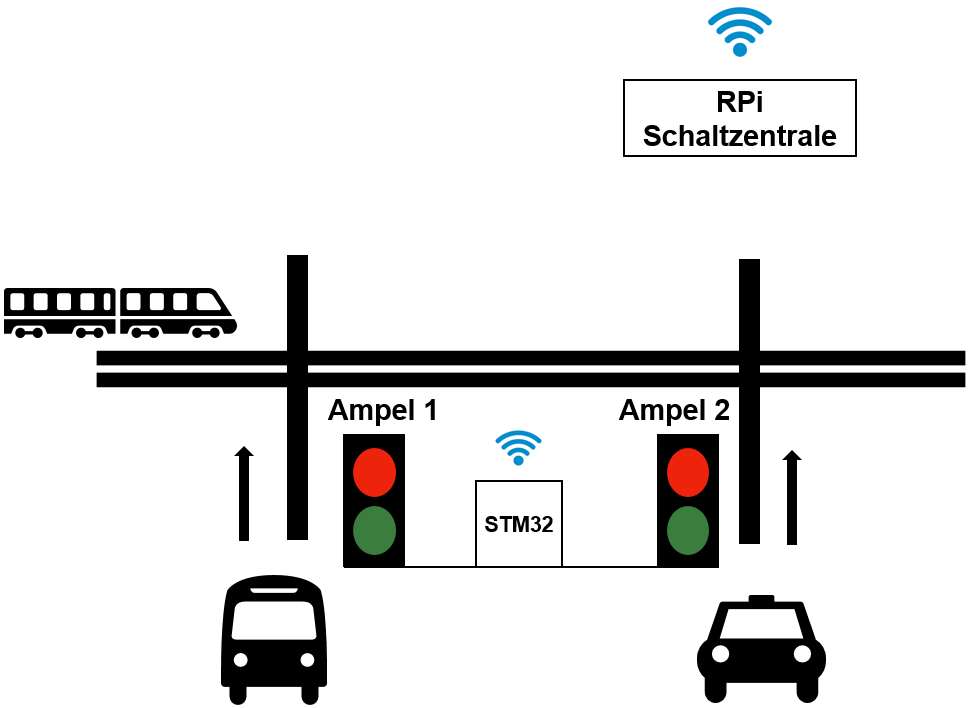
\includegraphics[height=50mm;left=50mm]{images/system}
	\centering
	\caption{system description}
	\label{fig:system}
\end{figure}

\paragraph
{
The adaptive cruise control (acc) system consists of two nodes, node1, and node2. The nodes are connected
by a (FIXME: encrypted/authenticated/both) bluetooth link.
}

\paragraph
{
	node1 hosts two ultrasonic proximity sensors which shall detect objects in the front of a virtual car. If
	a request from node2 arrives, node1 reads both sensors, compares their readings for consistency and plausibility,
	then returns the readings to node1. The returned message also contains information about the consistency and
	plausibility status of the readings.
	FIXME: The fault hypothesis is that one of these sensors can fail, but not both of them within a defined
	time span. We design node1 in such a way that it is fail-silent: It does not convey incrrect readings to node2,
	but it may convey no readings at all if the sensors are failing.
}

\paragraph
{
	node2 represents the steering wheel ECU of the virtual car. It is connected to a control panel by which the virtual 
	vehicle can be accelerated/decelerated. Another switch turns the adaptive cruise control on or off.
	A display shows the current speed of the car and gives status information on whether acc is on or off.
	Moreover it shows an alarm if the acc detects an error.
	FIXME: We can solve the status/speed/alarm/input requirements with a touch screen, e.g. 
	\href{https://www.berrybase.de/3-5-ips-display-fuer-raspberry-pi-mit-resistivem-touchscreen} {such a device}.
}

